%        File: TanhSummation.tex
%     Created: Mon Jun 20 04:00 AM 2022 E
% Last Change: Mon Jun 20 04:00 AM 2022 E
%
\documentclass[a4paper]{article}
\usepackage{pgfplots}
\usetikzlibrary{calc}
\usepackage{amsmath}
\begin{document}

\begin{titlepage}
    \title{Tanh Summation Method}
    \author{
        Jeffrey Severino \\
        Dr. Ray Hixon \\
        Toledo, OH 43606 \\
        email: jseveri@rockets.utoledo.edu \\
    }
\maketitle 
    
\end{titlepage}
\section{Introduction}

Knupp's Code Verification by the Method of Manufactured Solution (MMS) provides 
``guidelines'' for creating a manufactured solution (MS) such that the observed
order of accuracy will approach a theoretical order of accuracy as the number
of grid points are reduced from one iteration to the next. While these guidelines
offer a road map, there are choices that are left to the investigator that would
benefit from additional examples. The first guideline gives the user a free
choice of the MS as long as it s smooth. The benefit of the tanh summation method 
(TSM) reduces the difficuly in defining a sufficient MS by providing 
a general summation formulation that allows the user to Vary the number of 
terms in the MS, and the MS behavior without manually changing terms in the MS
symbolic expression. 

The general form of the MS will be a summation of $tanh$ bounded between zero
and one. A MS created with the TSM can provide a significant result for
a numerical differencing/integration technique by having inflection points of each
$tanh$ at various locations along the domain, giving a stair like slope.
While the TSM can add a layer of complexity to the MS that may not be needed, 
writing the formulation in a summation lends itself to iterative loops that can 
be coded, thus reducing the need for manual adjust of the MS, 
which can be an initial hurdle when performing MMS.


\section{General form of a Hyperbolic Tangent}

\begin{equation}
    R = A tanh(B(x-C)) 
    \label{eqn:1}
\end{equation}

\begin{equation}
    L = A tanh(B(C-E)) 
    \label{eqn:2}
\end{equation}
\begin{equation}
    y = R + L + D
    \label{eqn:3}
\end{equation}
where 
\begin{itemize}
    \item $R \equiv$ The value of the hyperbolic tangent. The variable $R$ represnts
        a ``right'' facing hyperbolic tangent kink.
    \item $A \equiv$ magnitude factor that increases or decreases the asymptotic
        limits $\lim_{x \to -\infty} = -1$ $\lim_{x \to \infty} = 1$
    \item $B \equiv$ ``steepness'' of the hyperbolic tangent
    \item $C \equiv$ The shift in inflection point of the hyperbolic tangent along the $
        x$ axis 
    \item $D \equiv$ The shift in inflection point of the hyperbolic tangent along the $
        y$ axis 
    \item $E \equiv$  $x_{i=i_{max}}$
    \item $x$ The domain. $x_i$ is used to indicate grid point indicies.
\end{itemize}
The idea is to sum up an arbitrary amount of tangents that will be bounded by zero
and one. 

\begin{figure}
    \centering
    \resizebox{\columnwidth}{!}{
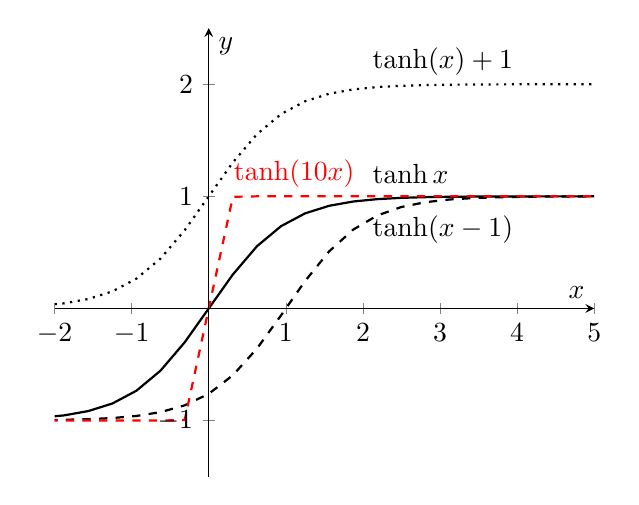
\begin{tikzpicture}
    \begin{axis}[
        xmin=-2, xmax=5,
        ymin=-1.5, ymax=2.5,
        axis lines=center,
        axis on top=true,
        domain=-2.5:5,
        ylabel=$y$,
        xlabel=$x$,
        ]

        \addplot [mark=none,draw= black, thick] {tanh(\x)};
        \node [right, black ] at (axis cs: 2,1.2) {$ \tanh x$};


        \addplot [mark=none,draw=black, dashed, thick] {tanh(\x - 1)};
        \node [right, black] at (axis cs: 2,0.7) {$ \tanh (x - 1)$};



        \addplot [mark=none,draw=red, dashed, thick] {tanh(10*\x)};
        \node [right, red] at (axis cs: 0.2,1.2) {$ \tanh (10x )$};



        \addplot [mark=none,draw=black, dotted, thick] {tanh(\x) + 1};
        \node [right, black] at (axis cs: 2,2.2) {$ \tanh (x) + 1$};

    \end{axis}
\end{tikzpicture}}
\end{figure}


Now the goal is to generalize this formulation such that we can add up terms.
$A$ is determined by setting a maximum amplitude for each $tanh$ function by
$A = A_{max}/n$. Note that amplitude can be different for each term but is chosen
to be the same. A parameter $\hat{x} = (x - x_{min})/ (x_{max} - x_{min}$ scales the domain to be between the  
minimum and maximum bounds.


\begin{equation}
    R_{ij} = A tanh(B(x_i-C_j)) 
    \label{eqn:1}
\end{equation}

\begin{equation}
    L_{j} = A tanh(B(C_j-E)) 
    \label{eqn:2}
\end{equation}
\begin{equation}
    y = \sum_{j = 1}^{n}  R_{ij} + \sum_{j = 1}^{n}L + D
    \label{eqn:3}
\end{equation}
The function \verb|TanhMethod| does this procedure. 

Setting $A = 1/16$ and $C_1  = 0$ , $C_2 = 0.75$ , $C_3 = 1$ , $D = 1$, $E = 1$  and 
$B = 10$


\begin{equation}
    \sum_{j = 1}^{3} R_{ij} = 1/16 tanh(10(\hat{x}_i))  + 1/16 tanh(10(\hat{x}_i-0.75)) + 1/16 tanh(10(\hat{x}_i-1))
    \label{eqn:1}
\end{equation}

\begin{equation}
    \sum_{j = 1}^{3} L_{j} = 1/16 tanh(10(-1))  + 1/16 tanh(10(0.75 - 1)) + 1/16 tanh(10(1-1))
    \label{eqn:1}
\end{equation}

The simplified expression becomes,
\begin{equation}
    y = \frac{1}{16}\tanh\left(\frac{100}{9}r - \frac{100}{9}\right) + \frac{1}{16}\tanh\left(\frac{100}{9}r -\frac{55}{9}\right) + \frac{1}{16}\tanh\left(\frac{100}{9}r -\frac{10}{9} \right) + \frac{7}{8}
\end{equation}


\begin{figure}
    \centering
    \resizebox{\columnwidth}{!}{
% This file was created with tikzplotlib v0.10.1.
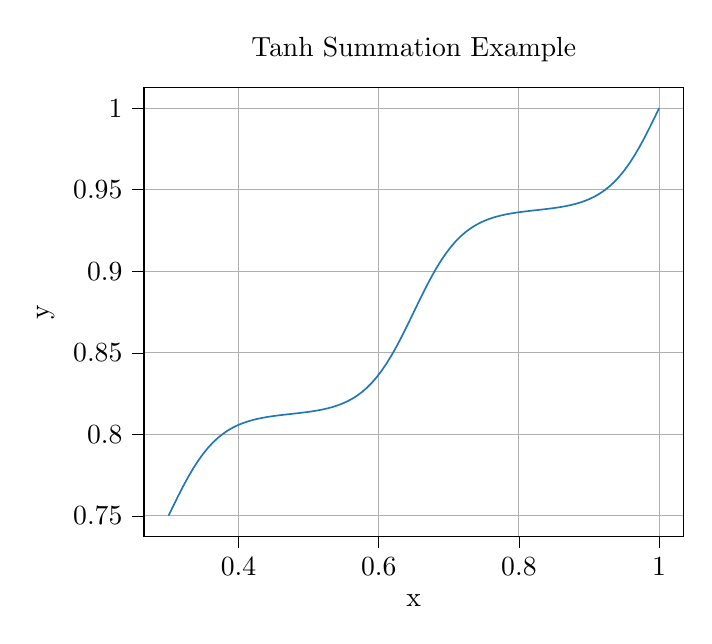
\begin{tikzpicture}

\definecolor{darkgray176}{RGB}{176,176,176}
\definecolor{steelblue31119180}{RGB}{31,119,180}

\begin{axis}[
tick align=outside,
tick pos=left,
title={Tanh Summation Example},
x grid style={darkgray176},
xlabel={x},
xmajorgrids,
xmin=0.265, xmax=1.035,
xtick style={color=black},
y grid style={darkgray176},
ylabel={y},
ymajorgrids,
ymin=0.737511917481587, ymax=1.01249943250088,
ytick style={color=black}
]
\addplot [semithick, steelblue31119180]
table {%
0.3 0.750011349982464
0.307070707070707 0.756304367923548
0.314141414141414 0.762471427961815
0.321212121212121 0.768396284241735
0.328282828282828 0.773980954849054
0.335353535353535 0.779151246168556
0.342424242424242 0.78385900159005
0.349494949494949 0.788081304133098
0.356565656565657 0.791817372304981
0.363636363636364 0.795084105493723
0.370707070707071 0.797911187966577
0.377777777777778 0.80033644822293
0.384848484848485 0.802401902498815
0.391919191919192 0.804150668035091
0.398989898989899 0.805624753143957
0.406060606060606 0.806863623924088
0.413131313131313 0.807903399550648
0.42020202020202 0.808776520778204
0.427272727272727 0.809511752175423
0.434343434343434 0.810134404577104
0.441414141414141 0.810666691986701
0.448484848484848 0.811128162249061
0.455555555555556 0.811536161419119
0.462626262626263 0.81190630759737
0.46969696969697 0.812252961565677
0.476767676767677 0.812589689584715
0.483838383838384 0.812929718947268
0.490909090909091 0.813286389915873
0.497979797979798 0.813673608902656
0.505050505050505 0.814106307344292
0.512121212121212 0.814600908628971
0.519191919191919 0.815175801361504
0.526262626262626 0.815851810708233
0.533333333333333 0.816652649865894
0.54040404040404 0.817605320080265
0.547474747474747 0.81874040944222
0.554545454545454 0.820092217733837
0.561616161616162 0.82169860781786
0.568686868686869 0.82360045643945
0.575757575757576 0.825840555061835
0.582828282828283 0.828461805118854
0.58989898989899 0.831504577298413
0.596969696969697 0.835003179865009
0.604040404040404 0.838981523240156
0.611111111111111 0.84344828154901
0.618181818181818 0.848392114910775
0.625252525252525 0.853777768834061
0.632323232323232 0.859544011154562
0.639393939393939 0.865604291561671
0.646464646464646 0.871850642171087
0.653535353535354 0.878160707811378
0.660606060606061 0.884407058420794
0.667676767676768 0.890467338827903
0.674747474747475 0.896233581148404
0.681818181818182 0.90161923507169
0.688888888888889 0.906563068433455
0.695959595959596 0.911029826742308
0.703030303030303 0.915008170117455
0.71010101010101 0.918506772684051
0.717171717171717 0.92154954486361
0.724242424242424 0.92417079492063
0.731313131313131 0.926410893543014
0.738383838383838 0.928312742164604
0.745454545454545 0.929919132248627
0.752525252525252 0.931270940540244
0.75959595959596 0.9324060299022
0.766666666666667 0.93335870011657
0.773737373737374 0.934159539274231
0.780808080808081 0.93483554862096
0.787878787878788 0.935410441353493
0.794949494949495 0.935905042638172
0.802020202020202 0.936337741079808
0.809090909090909 0.936724960066591
0.816161616161616 0.937081631035197
0.823232323232323 0.937421660397749
0.83030303030303 0.937758388416787
0.837373737373737 0.938105042385094
0.844444444444444 0.938475188563345
0.851515151515152 0.938883187733403
0.858585858585859 0.939344657995763
0.865656565656566 0.939876945405361
0.872727272727273 0.940499597807041
0.87979797979798 0.94123482920426
0.886868686868687 0.942107950431816
0.893939393939394 0.943147726058376
0.901010101010101 0.944386596838507
0.908080808080808 0.945860681947373
0.915151515151515 0.947609447483649
0.922222222222222 0.949674901759534
0.929292929292929 0.952100162015887
0.936363636363636 0.954927244488741
0.943434343434343 0.958193977677483
0.950505050505051 0.961930045849366
0.957575757575758 0.966152348392414
0.964646464646465 0.970860103813908
0.971717171717172 0.97603039513341
0.978787878787879 0.981615065740729
0.985858585858586 0.987539922020649
0.992929292929293 0.993706982058916
1 1
};
\end{axis}

\end{tikzpicture}

}
\end{figure}
\section{Appendix}
\begin{verbatim}
# ========= Packages ========
import sympy as sp 
import numpy as np
def TanhMethod(n,B,r_min,r_max):
    # inputs: 
    #   n - number of tanh functions
    #   B - the slope around the inflection point
    
    # outputs:     
    # initialize lists for the tanh function
    RightKink  = []
    LeftKink   = []
   
    # symbolic variables needed for this function
    r = sp.Symbol('r')
    
    # rescaling the radius (redundant but needed for BC Fairing Function)
    r_hat = (r - r_min)/(r_max - r_min)    
    
    # amplitude for each wave
    A          = []
    
    # maximum allowed amplitude 
    max_amplitude = 0.25
   
    # vertical shift along the y axis
    # one is chosed to keep the inflection points above 
    # zero
    S_vertical = 1
    
    # rj is the list of inflection point locations
    rj = list(np.linspace(1,0,n))


    
    # messages for error and warning checking 
    warning_mssg = {1:'Warning: Total Amplitude exceeds maximum ', \
                    2:'Warning: Function is negative'}
    
    # getting amplitude for each kink
    for i in range(len(rj)):
        # 
        A.append(max_amplitude/(len(rj)+1))
        if sum(A) > max_amplitude:
            sys.exit(str(warning_mssg[1]))
    
    # defining kinks and antikinks
    for j in range(len(rj)):
        RightKink.append( A[j]*sp.tanh(B*( r_hat    - rj[j] )) )
        LeftKink.append(  A[j]*sp.tanh(B*( rj[j]- rj[0] )) )   
    
    f = sum(LeftKink) + sum(RightKink) + S_vertical
    print(A)
    return f

\end{verbatim}
\end{document}


